\documentclass[a4paper,twoside,phd]{BYUPhys}
% The BYUPhys class is for producing theses and dissertations
% in the BYU Department of Physics and Astronomy.  You can supply
% the following optional arguments in the square brackets to
% specify the thesis type:
%
%   senior  : Produces the senior thesis preliminary pages (default)
%   honors  : Produces the honors thesis preliminary pages
%   masters : Produces the masters thesis preliminary pages
%   phd     : Produces the PhD dissertation preliminary pages
%
% The default format is appropriate for printing, with blank pages
% inserted after the preliminary pages in twoside mode so you can
% send it directly to a two-sided printer. However, for ETD
% submission the blank pages need to be removed from the final output.
% The following option does this for you:
%
%   etd     : Produces a copy with no blank pages in the preliminary section.
%             Remove this option to produce a version with blank pages inserted
%             for easy double sided printing.
%
% The rest of the class options are the same as the regular book class.
% A few to remember:
%
%   oneside : Produces single sided print layout (recommended for theses less than 50 pages)
%   twoside : Produces double sided print layout (the default if you remove oneside)
%
% The BYUPhys class provides the following macros:
%
%   \makepreliminarypages : Makes the preliminary pages
%   \clearemptydoublepage : same as \cleardoublepage but doesn't put page numbers
%                           on blank intervening pages
%   \singlespace          : switch to single spaced lines
%   \doublespace          : switch to double spaced lines
%
% --------------------------- Load Packages ---------------------------------

% The graphicx package allows the inclusion of figures.  Plain LaTeX and
% pdfLaTeX handle graphics differently. The following code checks which one
% you are compiling with, and switches the graphicx package options accordingly.
\usepackage{ifpdf}
\ifpdf
  \usepackage[pdftex]{graphicx}
\else
  \usepackage[dvips]{graphicx}
\fi

%%%%%%%%%%%%%%%%%%%%%%%%%%%%%%%%%%%%%%%%%%%%%%%%%%%%%%%%%%%%%%%%%%
% Edited : Beeshanga
%
% If you need to include any code in the text use this package
% \usepackage{listings}
% It can be used to make key words bold, add colours, etc. Refer
% to http://en.wikibooks.org/wiki/LaTeX/Packages/Listings for
% more information.
%
% For theorems, propositions, proofs and assumtions use this
% package
% \usepackage{amsthm}
% For more information refer to the following website
% http://en.wikibooks.org/wiki/LaTeX/Theorems
%
%%%%%%%%%%%%%%%%%%%%%%%%%%%%%%%%%%%%%%%%%%%%%%%%%%%%%%%%%%%%%%%%%%

% The fancyhdr package allows you to easily customize the page header.
% The settings below produce a nice, well separated header.
\usepackage{fancyhdr}
  \fancyhead{}
  \fancyhead[LO]{\slshape \rightmark}
  \fancyhead[RO,LE]{\textbf{\thepage}}
  \fancyhead[RE]{\slshape \leftmark}
  \fancyfoot{}
  \pagestyle{fancy}
  \renewcommand{\chaptermark}[1]{\markboth{\chaptername \ \thechapter. #1}{}}
  \renewcommand{\sectionmark}[1]{\markright{\thesection \ #1}}


% The cite package cleans up the way citations are handled.  For example, it
% changes the citation [1,2,3,6,7,8,9,10,11] into [1-3,6-11].  If your advisor
% wants superscript citations, use the overcite package instead of the cite package.
\usepackage{cite}

% The makeidx package makes your index for you.  To make an index entry,
% go to the place in the book that should be referenced and type
%  \index{key}
% An index entry labeled "key" (or whatever you type) will then
% be included and point to the correct page.
%\usepackage{makeidx}
%\makeindex

% The url package allows for the nice typesetting of URLs.  Since URLs are often
% long with no spaces, they mess up line wrapping.  The command \url{http://www.physics.byu.edu}
% allows LaTeX to break the url across lines at appropriate places: e.g. http://www.
% physics.byu.edu.  This is helpful if you reference web pages.
\usepackage{url}
\urlstyle{rm}

% If you have a lot of equations, you might be interested in the amstex package.
% It defines a number of environments and macros that are helpful for mathematics.
% We don't do much math in this example, so we haven't used amstex here.
\usepackage{amsmath}
\usepackage{amssymb}
\usepackage{subfigure}
\usepackage{cite}
\usepackage{amsxtra}
\usepackage{amsfonts}
\usepackage{graphicx}
\usepackage{multirow} % This is package for multi-rows in tables added on 7th July 2009 by Arif
%\usepackage{setspace}

% The caption package allows us to change the formatting of figure captions.
% The commands here change to the suggested caption format: single spaced and a bold tag
\usepackage[labelfont=bf,labelsep=colon]{caption}%[2008/04/01]
 \DeclareCaptionFormat{suggested}{\singlespace#1#2#3\par\doublespace}
 \captionsetup{format=suggested}


\usepackage{array}
\usepackage{multirow}
\usepackage{verbatim}
\usepackage{enumerate}

% Defining the symbols




% The hyperref package provides automatic linking and bookmarking for the table
% of contents, index, equation references, and figure references.  It must be
% included for the BYU Physics class to make a properly functioning electronic
% thesis.  It should be the last package loaded if possible.
%
% To include a link in your pdf use \href{URL}{Text to be displayed}.  If your
% display text is the URL, you probably should use the \url{} command discussed
% above.
%
% To add a bookmark in the pdf you can use \pdfbookmark.  You can look up its usage
% in the hyperref package documentation
\usepackage[bookmarksnumbered,pdfpagelabels=true,plainpages=false,colorlinks=true,
            linkcolor=black,citecolor=red,urlcolor=blue]{hyperref}

% My custom packages
\usepackage{float}


% ------------------------- Fill in these fields for the preliminary pages ----------------------------
%
% For Senior and honors this is the year and month that you submit the thesis
% For Masters and PhD, this is your graduation date
  \Year{2020}
  \Month{October 22,}
  \Author{James Ridey}

% If you have a long title, split it between two lines. The \TitleBottom field defines the second line
% A two line title should be an "inverted pyramid" with the top line longer than the bottom.
  \TitleTop{Reduction of neural network complexity through}
  \TitleBottom{stochastic numbers} % edited Beeshanga
 \DegreeTitle{Bachelor of Engineering
 \\ Software Engineering} % edited Beeshanga

% Your research advisor
 \Advisor{Supervisor: Associate Professor Tara Hamilton}

% The department undergraduate research coordinator
%  \UgradCoord{A}

% The representative of the department who will approve your thesis (usually the chair)
%  \DepRep{B}

% Acknowledge those who helped and supported you

  \Acknowledgments{
  \vspace{-1.5cm}
    \noindent I would like to acknowledge and thank, Tara Hamilton and Alan Kan for their support and advice during my thesis.
  }


% The title of the department representative
%  \DepRepTitle{Chair}
  \Statement{
    \noindent I, James Ridey, declare that this report, submitted as part of the requirement for the award of Bachelor of Engineering in the School of Engineering, Macquarie University, is entirely my own work unless otherwise referenced or acknowledged. This document has not been submitted for qualification or assessment an any academic institution.
    \vspace{0.5cm}

    \noindent     Student's Name: James Ridey

    \vspace{0.25cm}

    \noindent Student's Signature: James Ridey

    \vspace{0.25cm}

    \noindent     Date: 7/6/2019
    }

% The text of your abstract
\Abstract{
\vspace{-1.5 cm}
Neural networks considered a core foundation of machine learning, has recently ballooned into a large framework that requires vast amounbts of computing resources and time. Here, we examine how to improve these networks, hoping to achieve networks that can calculate the same result with less training time and/or resources using ideas such as stochastic numbers and probalistic results.
}



% Statement of Candidate



\fussy

\begin{document}

 % Start page counting in roman numerals
 \frontmatter

 % This command makes the formal preliminary pages.
 % You can comment it out during the drafting process if you want to save paper.

 \makepreliminarypages


%\clearemptydoublepage
\doublespace
%\include{Publications/publications}

% \clearemptydoublepage
%\include{Organization/organization}

 \clearemptydoublepage
\singlespace
 % Make the table of contents.
 \tableofcontents

\clearemptydoublepage
% Make the list of figures
\listoffigures

\clearemptydoublepage
% Make the list of tables
\listoftables

\clearemptydoublepage

% Start regular page counting at page 1
\mainmatter
%
\chapter{Introduction}
\label{chap:Introduction}


\section{Neural networks: introduction}
Neural networks are the core structure of what many believe to be the next step in computing, machine learning. 


\chapter{Background and Related Work}
\label{chap:LitReview}

\section{Neural networks: explanation}
Neural networks are a very rough simulation of how the neurons in a human brain actually work. The most common form of a neural network in the feed forward model where the inputs are passed to the neural network and it outputs an answer. The feed forward model consists of an input layer, hidden layers and an output layer each of these layers are composed of varying amounts of neurons depending on the complexity of the data that is trying to be learned. More models of neural networks exist which aim to memorise or improve the feed forward model, however the feed forward model is incredibly ubiquidious and is the main driving force behind machine learning in the industry. 

To understand what each layer in a neural network is doing, it is first necessary to understand what a neuron is doing. A neuron is comprised of inputs, a set of weights and one output, as shown below.
\begin{figure}[H]
\centering
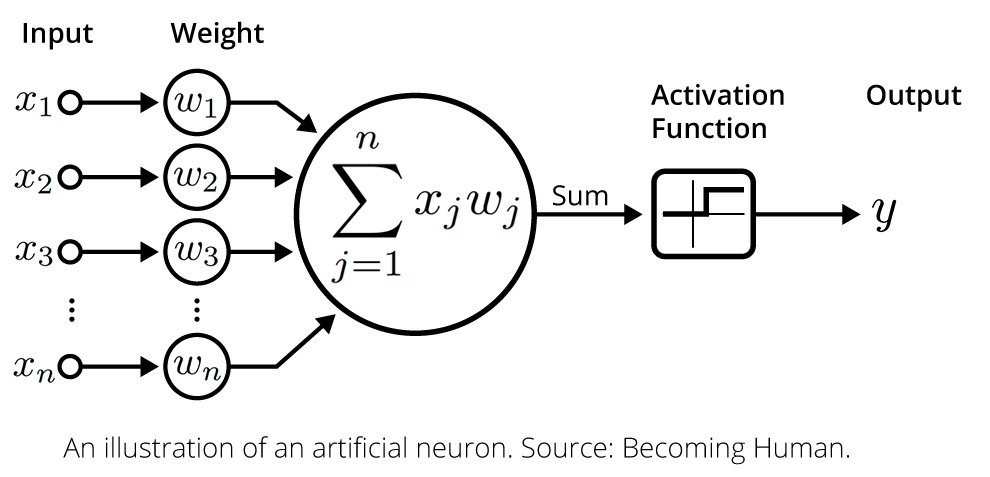
\includegraphics[width=8cm]{pictures/neuron_model.png}
\caption{Neuron model.}
\label{fig:neuron_model}
\end{figure}

Neurons are fed a set of data through its inputs which are multiplied by a specific weight, all of these numbers are then added up and fed to an activation function. An activation function is a function that maps the input to a value between 0 and 1, a commonly used activation function is the sigmoid function, numbers in the positive infinity direction become increasingly closer to 1, while numbers in the negative infinity direction become increasing closer to 0.
\begin{figure}[H]
\centering
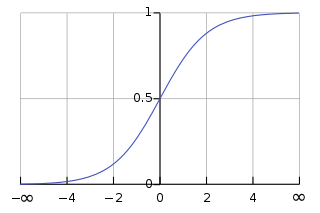
\includegraphics[width=8cm]{pictures/sigmoid.png}
\caption{Sigmoid graph.}
\label{fig:sigmoid}
\end{figure}

Next is neural network layers where the most common layer is the dense layer, in this layer every neuron connects to every other neuron in the previous layer.
\begin{figure}[H]
\centering
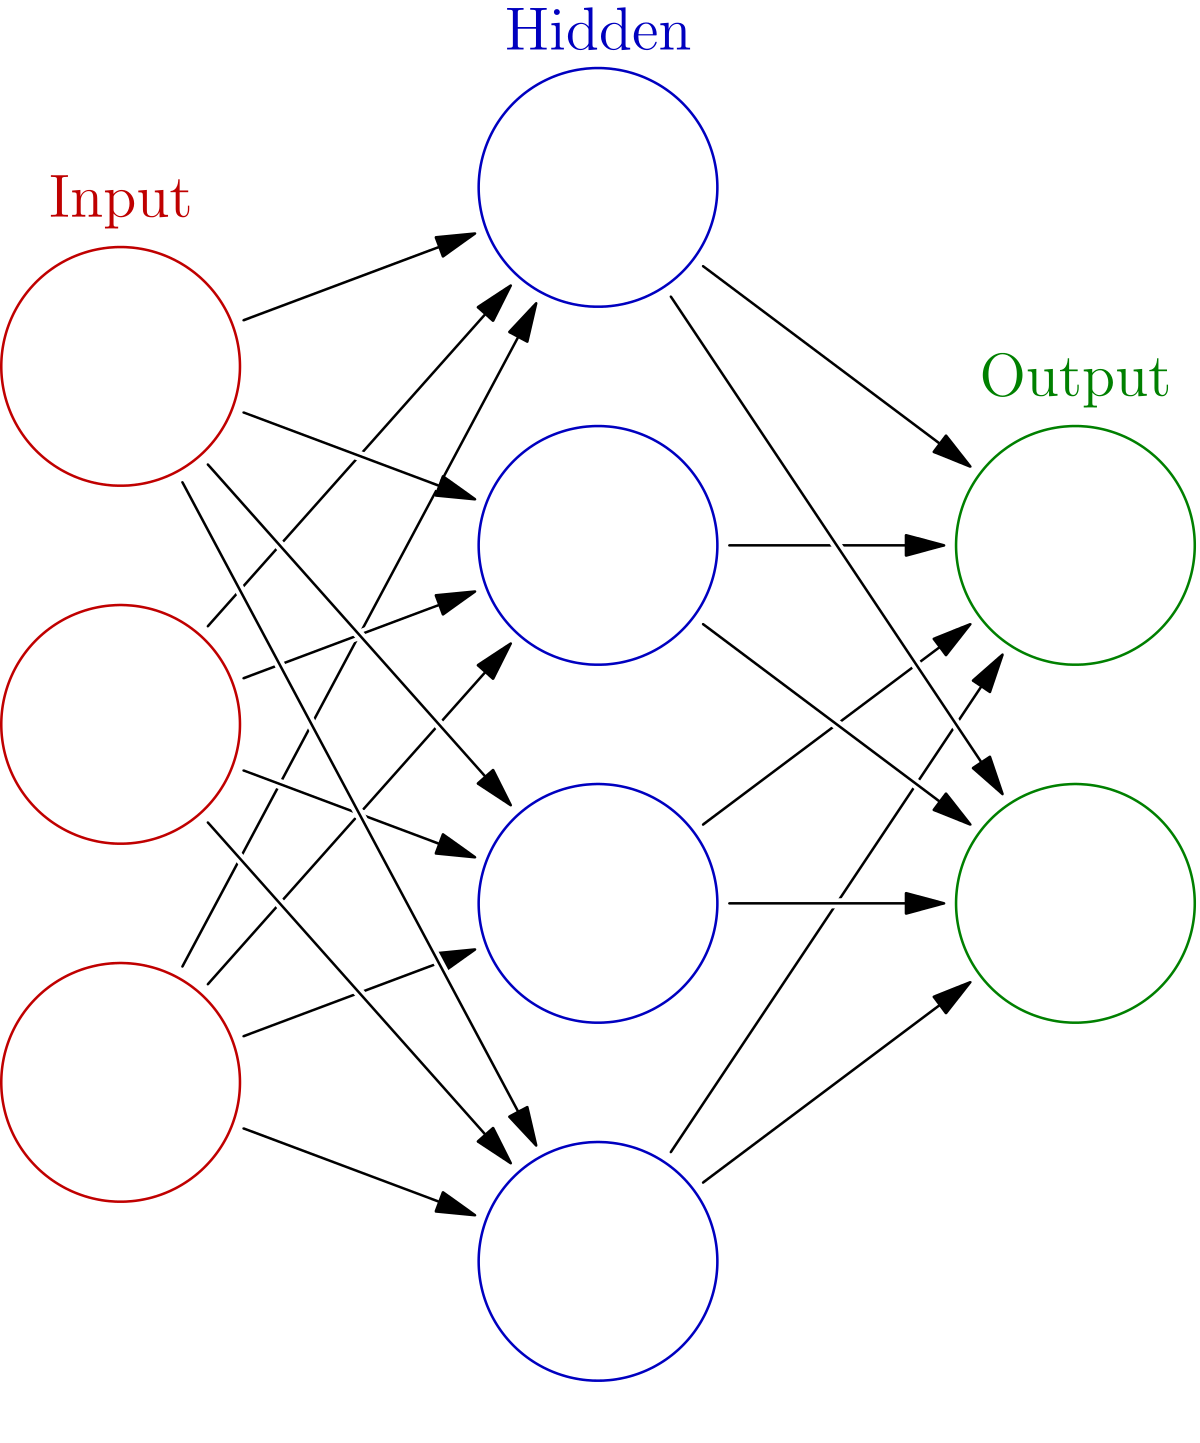
\includegraphics[width=8cm]{pictures/neural_network_model.png}
\caption{Neural network model.}
\label{fig:neural_network_model}
\end{figure}

Each circle in this figure represents a neuron and each line in this figure represents a connection between these 2 neurons. By manipulating the weights in the neural network, we change what each neuron calculates and outputs as part of its activation function. In doing so, we now have a framework of which for any given input, the neural network can generate any output (given the right weights), regardless of the complexity of the output\cite{nielsen_2018}. 

\subsection{Training}
The next question about neural networks are then how are the weights trained for a given input.
TODO

\section{Stochastic numbers}

\section{Tensorflow}
Tensorflow is a machine learning framework primarily written in Python. It was released by Google under the Apache License 2.0 on November 9th, 2015. The Tensorflow network employs the idea of creating a neural network model which is then compiled before being handed off to the appropiate processing unit be it CPU or GPU, this is in contrast to other machine learning frameworks like PyTorch that generate their models dynamically on the fly which results in a small performance hit.

Tensorflow continues to grow in support with new frameworks like Kera that aim to simplify common operations and overall streamline the process and show no signs of stopping with a stable release only 2 months ago.

\section{MNIST dataset}
The MNIST dataset is a commonly used dataset for machine learning that consists of 70,000 images of handwritten digits (60,000 training images and 10,000 test images) and the associated labels for each of these images. The dataset is commonly choosen due to its simplicity and many frameworks support it out of the box.

Another common reason that MNIST is choosen is to demonstrate the accuracy of neural networks over more traditional statistical analysis such as linear classifiers and K-nearest neighbours, both of which score around an error rate of 12\% and 5\% respectively\cite{lecun-98} as compared to a simple neural network of 3 layers which can score around 3.05\%\cite{lecun-98}.

However this dataset is not without its faults, there are quite a number of images that are dubiously labeled.
\begin{figure}[H]
\centering
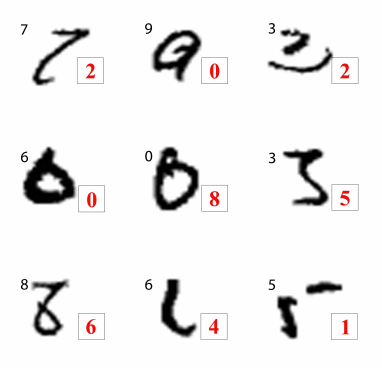
\includegraphics[width=8cm]{pictures/mnist_incorrect.png}
\caption{Samples of ambigious digits.}
\label{fig:incorrect_mnist}
\end{figure}
The dataset is also often constructed as too small and too simple, consisting of only 70,000 images of greyscale images. Compared to datasets such as CIFAR10 which has the same amount of images but 32x32 color images or another dataset like ImageNet consisting of 1,331,167 images, MNIST is certainly behind. However MNIST has been used and is continued to be used as a way to quickly validate a machine learning algorithm before moving on to larger more complicated datasets that take much more time to compute.


\chapter{Preliminary results}
\section{Stochastic numbers}

\chapter{Conclusions and Future Work}
\label{chap:Conclusions}


\section{Conclusions}
\label{sec:ConclusionsConclusions}

This



\clearemptydoublepage
\chapter{Abbreviations}
\label{chap:abbreviations}

\begin{tabbing}

AWGN \qquad \qquad \= Additive White Gaussian Noise\\
SC \> Stochastic numbers\\
NN \> Neural network \\
\end{tabbing}

%\phantomsection \addcontentsline{toc}{chapter}{Index}
% \renewcommand{\baselinestretch}{1} \small \normalsize
% \printindex

\appendix
\chapter{name of appendix A}
\section{Overview}
here is the Overview of appendix A ...
\section{Name of this section}
here is the content of this section ...
\chapter{name of appendix B}
\section{Overview}
here is the Overview of appendix B ...
\section{Name of this section}
here is the content of this section ...

%\input{Bibliography/biblio3}
\bibliographystyle{IEEEtran}
%\bibliographystyle{acm}
\bibliography{my_reference}
%\bibliography{Bibliography/biblio4}


\end{document}
